
\section{mclique2g.rb Generate Maximal Clique\label{sect:mclique2g}}

This command enumerates nodes of each maximal clique  \footnote{refer to section \ref{sect:mclique} on the definition of maximal clique.} from general graph (this is referred to as ``original graph" below) to create new graph  (referred to as maximal clique graph). 
An edge is added to connect common nodes between cliques. 

An example is shown as follows. 
Graph in Figure \ref{fig:clique2g_1} contains 4 maximal cliques, Figure \ref{fig:clique2g_2} shows the new graph generated from the original graph. 
Node $0$ corresponds to clique \{$a,b,c,d$\} in Figure \ref{fig:clique}, node $1$ corresponds to \{$d,e,f$\}, and finally node $2$ corresponds to \{$e,f,h$\}. Similarly, node $3$ corresponds to \{$e,f,h$\}. 
 
Node $0$ and $1$ of maximal clique graph has 1 ($d) common node with the original graph, thus an edge is extended to node  $0$ and $1$, with a weight of 1. 
Similarly, $1$ and $2$ contains two common nodes ($e,f$), an edge is extended to node $1$ and $2$, and the weight becomes 2. 
On the other hand, $0$ and $2$ do not have common nodes, an edge is not extended between node  $0$ and $2$. 

\begin{figure}[htbp]
\begin{center}
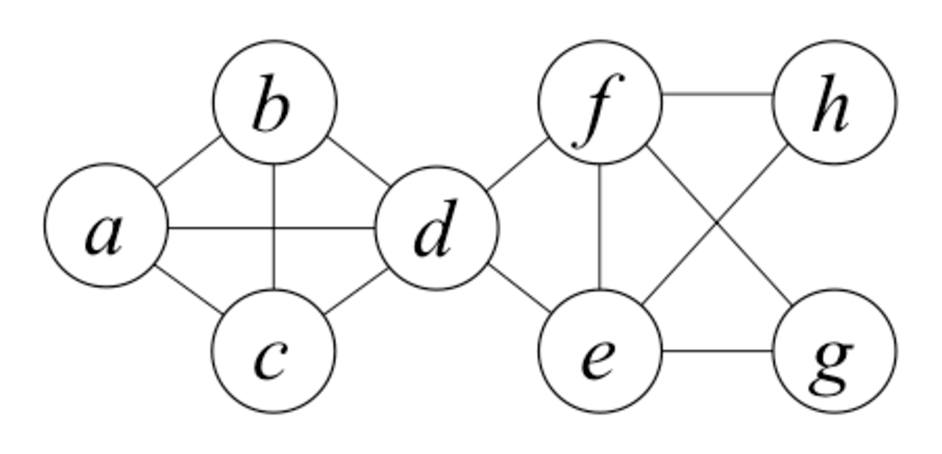
\includegraphics[scale=0.5]{./clique2g_1.eps}
\caption{Contains 4 maximal cliques
\{$a,b,c,d$\}
\{$d,e,f$\}
\{$e,f,g$\}
\{$e,f,h$\}.

\label{fig:clique2g_1}
}
\end{center}
\end{figure} 

\begin{figure}[htbp]
\begin{center}
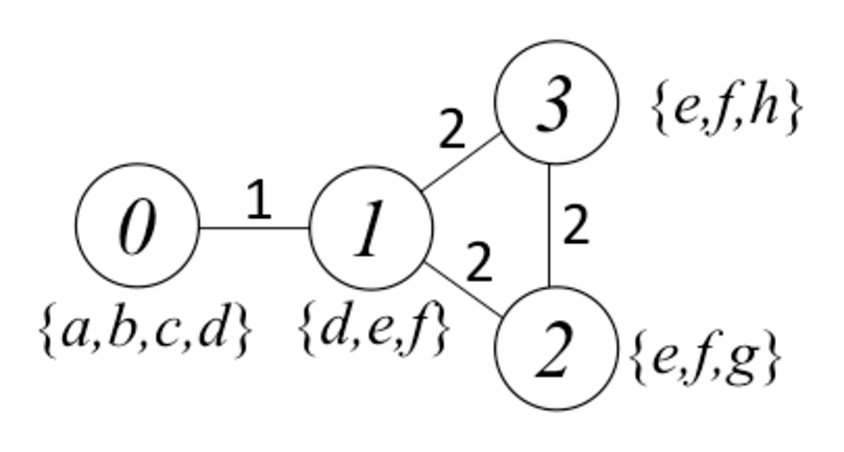
\includegraphics[scale=0.5]{./clique2g_2.eps}
\caption{Newly generated maximal clique graph\label{fig:clique2g_2}}
\end{center}
\end{figure} 

The original graph input data of this command is shown in  \ref{tbl: clique2g_1}, the data in CSV format, consisting of 2 columns, clique ID and node respectively. 
This data is corresponds to the data for mclique.rb command shown in \ref{sect:mclique} when \verb|-node| is specified. 

In addition, the output results of maximal cliques are created separately as node data (Table \ref{tbl:clique2g_2}) and edge data (Table\ref{tbl:clique2g_3}). 
The column \verb|weight| in the node data is the number of nodes that make up maximum clique. 
The column \verb|weight| in the edge data is the number of nodes that make up maximum clique.   


\begin{table}[htbp]
\begin{center}
\begin{tabular}{ccc}

\begin{minipage}{0.3\hsize}
\begin{center}
\caption{Original graph\label{tbl:clique2g_1}}
{\small
\begin{tabular}{cc}
\hline
id&node \\
\hline
0&a \\
0&b \\
0&c \\
0&d \\
1&d \\
1&e \\
1&f \\
2&e \\
2&f \\
2&g \\
3&e \\
3&f \\
3&h \\
\hline
\end{tabular} 
}
\end{center}
\end{minipage}

\begin{minipage}{0.3\hsize}
\begin{center}
\caption{Maximal clique graph (node data)\label{tbl:clique2g_2}}
{\small
\begin{tabular}{cccc}
\hline
node&weight \\
\hline
0&4 \\
1&3 \\
2&3 \\
3&3 \\
\hline
\end{tabular} 
}
\end{center}
\end{minipage}

\begin{minipage}{0.3\hsize}
\begin{center}
\caption{Maximal clique graph (edge data)\label{tbl:clique2g_3}}
{\small
\begin{tabular}{cccc}
\hline
node1&node2&weight \\
\hline
0&1&1 \\
1&2&2 \\
1&3&2 \\
2&3&2 \\
\hline
\end{tabular} 
}
\end{center}
\end{minipage}


\end{tabular} 
\end{center}
\end{table} 


\subsection{Format}
\begin{verbatim}
mclique2g.rb i= [id=] [f=] eo= no= [T=] [--help]

  Specification of file name 
  i=  : Clique file name
id= : Clique ID field name (default:"id")
  f=  : Field name of node from the clique generated (default:"node")
  eo= : Edge output filename 
  no= : Node output filename 

  Others
  T= : Working directory (default:/tmp)
  --help : Show help information 
\end{verbatim}

\subsection{Example}
\subsubsection*{例1: 基本例}

前節で解説した例。


\begin{Verbatim}[baselinestretch=0.7,frame=single]
$ more clique.csv
id,node
0,a
0,b
0,c
0,d
1,d
1,e
1,f
2,e
2,f
2,g
3,e
3,f
3,h
$ mclique2g.rb i=clique.csv eo=edge.csv no=node.csv id=id f=node
#END# /usr/bin/mclique2g.rb i=clique.csv eo=edge.csv no=node.csv id=id f=node
$ more edge.csv
node1,node2,weight
0,1,1
1,2,2
1,3,2
2,3,2
$ more node.csv
node,weight
0,4
1,3
2,3
3,3
\end{Verbatim}


